\documentclass{beamer}
\usepackage[utf8]{inputenc}

\usepackage{utopia} %font utopia imported
\usepackage{verbatim}

\usetheme{Madrid}
\usecolortheme{default}
\usepackage{graphicx}


%------------------------------------------------------------
%This block of code defines the information to appear in the
%Title page
\title[Wrangell] %optional
{Wrangell}

\subtitle{A DSL for Data-Wrangelling}

\author[Dana Iltis, Kenan Nalbant, Donald Pinckney] % (optional)
{Dana Iltis \and Kenan Nalbant \and Donald Pinckney}




%End of title page configuration block
%------------------------------------------------------------



%------------------------------------------------------------
%The next block of commands puts the table of contents at the 
%beginning of each section and highlights the current section:

\begin{comment}
\AtBeginSection[]
{
  \begin{frame}
    \frametitle{Table of Contents}
    \tableofcontents[currentsection]
  \end{frame}
}
\end{comment}
%------------------------------------------------------------


\begin{document}

%The next statement creates the title page.
\frame{\titlepage}

\begin{comment}
%---------------------------------------------------------
%This block of code is for the table of contents after
%the title page
\begin{frame}
\frametitle{Table of Contents}
\tableofcontents
\end{frame}
%---------------------------------------------------------
\end{comment}



%---------------------------------------------------------
%Changing visivility of the text
\begin{frame}
\frametitle{Data Wrangling: a time-consuming and tedious job}
Why do we need a DSL for data-wrangelling?
\begin{itemize}
    \item<1-> Wide variety of file formats
    \item<1-> Difficult to accomplish for users with minimal programming experience
    \item<1-> Often requires manual labor to create ad-hoc solutions
    %\item<2-> Text visible on slide 2
    %\item<3> Text visible on slides 3
    %\item<4-> Text visible on slide 4
\end{itemize}
\end{frame}

%---------------------------------------------------------

\section{Second section}

\begin{frame}
\frametitle{A Motivating Example}
Perhaps we want to remove sensitive information from a database

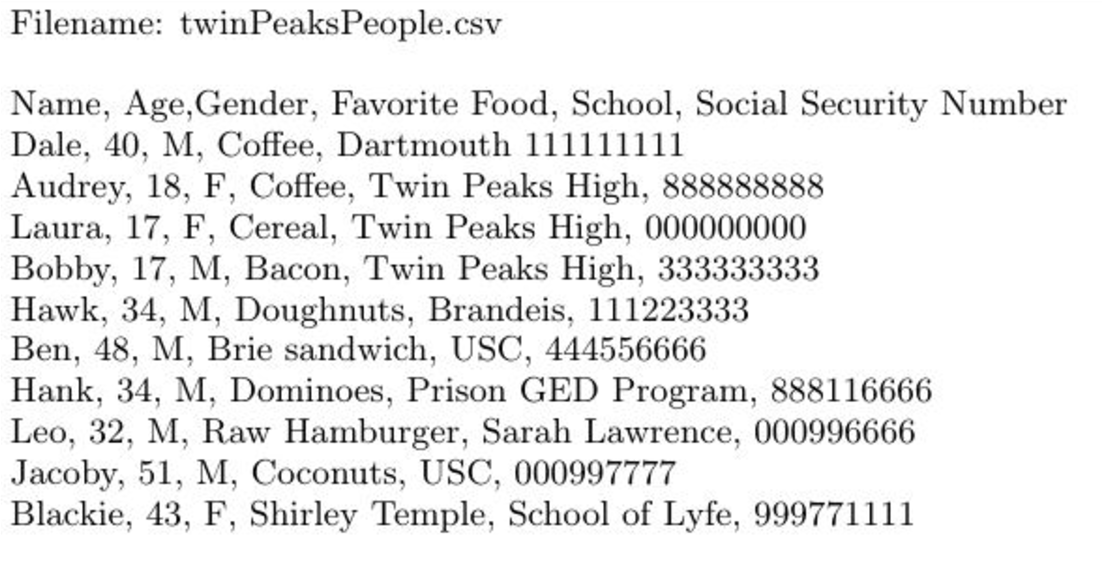
\includegraphics[scale=0.35]{screen}


\end{frame}

\section{Third Section}
\begin{frame}
\frametitle{Solution: Create a DSL}
Why create \textit{another} DSL 
\begin{itemize}
    \item<1-> We want ease of usage when it comes to this particular problem domain while still allowing for a lot of flexibility 
    \item<1-> Make common place tasks easier to accomplish and eliminate tedious boilerplate that writing an ad-hoc solution in another language would require 
    %\item<2-> Text visible on slide 2
    %\item<3> Text visible on slides 3
    %\item<4-> Text visible on slide 4
\end{itemize}
\end{frame}

\section{Fourth Section}
\begin{frame}
\frametitle{Introducing Wrangell}
Wrangell is a DSL which eliminates much of the boilerplate code that typically arises when data-munging.
\begin{itemize}
    \item<1> Based on a familiar Lisp-like syntax which while simple is very expressive.
    \item<1> Very extensible, arbitrary new file formats can be supported for input and output as long as functions which map to and from Wrangell's internal data representation are provided.
    \item<1>We have a working interpreter implemented in Haskell
\end{itemize}
\end{frame}


\section{Fifth Section}
\begin{frame}
\frametitle{Wrangell}
\begin{itemize}
    \item<1> Has a dynamic type system as with Lisp, but much more strict, with less implicit type coercions 
    \item<1> Additionally Wrangell supports polymorphic expressions, if the functions used in an expression can accept many different types so will the compound expression.
\end{itemize}
\end{frame}


\section{Sixth Section}
\begin{frame}
\frametitle{Wrangell}
\begin{itemize}
    \item<1> Wrangell also requires columns of the data set to have types.
    \item<1> All column transformations are type checked to guarantee type-soundness.
\end{itemize}
\end{frame}

\section{Seventh Section}
\begin{frame}
\frametitle{Why Haskell}
\begin{itemize}
    \item<1>  Because Haskell
is a functional language, we thought that data-wrangling,
with its emphasis on data transformations would be well suited and also an instructive experience on how to build large scale functional programs
\end{itemize}
\end{frame}

\section{Eighth Section}
\begin{frame}
\frametitle{Future Work}
\begin{itemize}
    \item<1> Currently the only supported type of input and output files are character delimited (e.g. CSV or TSV) so work can be done to make more file formats supported 
    \item<1> There is currently a degree of inefficiency with the current implementation of many of the internal data transformations which can absolutely be remedied 
\end{itemize}
\end{frame}



\section{Last Section}
\begin{frame}
\frametitle{Conclusion}
\begin{itemize}
    \item<1> Wrangell is a novel language which provides many primitives to easily deal with data-preprocessing tasks 
    \item<1> Wrangell additionally provides facilities to easily extend to new file types.
    \item<1> The type system on both Wrangell expressions and internal data tables allows for both expresiveness and safety 
\end{itemize}
\end{frame}




\end{document}